\documentclass[handout,11.5pt]{beamer}
\usepackage[numbers,sort&compress]{natbib}
\usepackage{amsmath,amssymb,amsfonts,amsthm}
\usepackage{algorithm,setspace}
\usepackage{algpseudocode}
\usepackage{caption}

\renewcommand{\algorithmicrequire}{\textbf{Input:}} 
\renewcommand{\algorithmicensure}{\textbf{Output:}} 

\setbeamertemplate{theorems}[numbered]
\setbeamerfont{frametitle}{series=\bfseries,parent=structure}
\newtheorem{assumption}{Assumption}


\usetheme{Boadilla}
\author[X. Li, C. Wu, \& Y. Huang]{Xiaopeng Li, Chenhao Wu \& Yihan Huang}
\title{Trajectory and Power Control for UAVs}
\institute[CUHK(SZ)]{The Chinese University of Hong Kong, Shenzhen}
\date{\today}

\begin{document}

\frame{\titlepage}

\begin{frame}
	\frametitle{Outline}
	\tableofcontents
\end{frame}

\section{Introduction}
\begin{frame}
	\frametitle{Introduction}
	Nowadays, UAVs are using widely in many areas.
\end{frame}

\section{Problem Formulation}
\begin{frame}
	\frametitle{Problem Formulation}
	To formulate this problem mathematically, we 
\end{frame}

\section{Main Strategies}
\begin{frame}
	\frametitle{Main Strategies}
	\begin{itemize}\itemsep4em
		\item<1-> Two main problems
		\begin{itemize}
			\item Large problem dimension
			\item Non-convex optimization
		\end{itemize}
		\item<2-> Two main strategies
		\begin{itemize}
			\item Heuristic dimension-reduced method
			\item Successive convex approximation (SCA)
		\end{itemize}
	\end{itemize}
\end{frame}


\begin{frame}
\frametitle{Main Strategies}
	\begin{block}<1->{Fly-hover-fly Strategy}
		The fly-hover-fly strategy is described as
		\begin{itemize}
			\item UAVs fly to the hovering location.
			\item UAVs hover over that location.
			\item UAVs return to the original position from the hovering location.
		\end{itemize}
	\end{block}
	\vskip 2\baselineskip
	\begin{assumption}<2->
		The whole time horizon $T$ is \alert{much longer} than the time UAVs need to fly to the hovering location.
	\end{assumption}
\end{frame}


\begin{frame}
\frametitle{Main Strategies}
	\begin{lemma}\label{lemma1}
		Assume all UAVs return to the initial locations, and the ascending and descending speed are equal, i.e., $V_A=V_D$. Denote one of the optimal solution of TPC problem as $\boldsymbol{q}^*$ and $\boldsymbol{p}^*$, then for all $k\in\mathcal{K},n\in\mathcal{N}_2^{N+2}$,
		\begin{equation}\label{lemma1eq}
			\boldsymbol{q}^*_{[:,k,n]} = \boldsymbol{q}^*_{[:,k,N+3-n]},\ \boldsymbol{p}^*_{[k,n]} = \boldsymbol{p}^*_{[k,N+3-n]}
		\end{equation}
	\end{lemma}
\end{frame}


\begin{frame}
\frametitle{Main Strategies}
	\begin{lemma}
		Using the same notations in {\rm Lemma \ref{lemma1}}, for some $M_0\in\{2,3,\ldots,N+1\}$ and $M\in\{2,3,\ldots,M_0\}$, we have
		\begin{equation}\label{lemma2eq}
			{R_s}_{[n]}\leq {R_s}_{[M]}={R_s}_{[M+1]}=\cdots={R_s}_{[M_0]},\ \forall\,n\in\mathcal{N}_2^M
		\end{equation}
		where $M_0$ is the time when the UAVs need to return from the hovering location, and $M$ is the time when UAVs arrives the hovering location. In particular, if $V_A=V_D$, $M_0=N+3-M$.
	\end{lemma}
\end{frame}


\begin{frame}
\frametitle{Main Strategies}
	\begin{itemize}
		\item<1-> Reformulation 1
		\begin{equation}\label{reformulation1}
			\begin{array}{cll}
			\max\limits_{\substack{\boldsymbol{p}_{[:,2:M]}, \\ \boldsymbol{q}_{[:,:,2:M]}, \\ M\in\mathcal{N}_2^{(N+1)/2}}}\quad & \sum\limits_{n=2}^{M}\sum\limits_{k=1}^K R_{[k,n]}(\boldsymbol{p},\boldsymbol{q}) \\[-20pt] &\qquad+\left(\frac{N+1}{2}-M\right)\sum\limits_{k=1}^KR_{[k,M]}(\boldsymbol{p},\boldsymbol{q}) \\
			s.t. \quad & (\ref{Eq1}),(\ref{Eq2.1}),(\ref{Eq2.2}),(\ref{Eq4}),\ \forall\,k\in\mathcal{K},n\in\mathcal{N}_2^M \\
			& (\ref{Eq3}),\ \forall\,k,j\in\mathcal{K},k<j,n\in\mathcal{N}_2^M
			\end{array}
		\end{equation}
		\item<2-> Reformulation 2
		\begin{equation}\label{reformulation2}
			\begin{array}{cl}
			\max\limits_{\substack{\boldsymbol{p}_{[:,2:M]}, \\ \boldsymbol{q}_{[:,:,2:M]} \\ M\in\mathcal{N}_2^{(N+1)/2}
			}} & \sum\limits_{n=2}^{M}\sum\limits_{k=1}^K R_{[k,n]}(\boldsymbol{p},\boldsymbol{q}) \\[-13pt] &\qquad+(\frac{N+1}{2}-M)R_s^* \\[5pt]
			s.t.  & (\ref{Eq1}),(\ref{Eq2.1}),(\ref{Eq2.2}),(\ref{Eq4}),\ \forall\,k\in\mathcal{K},n\in\mathcal{N}_2^M \\
			& (\ref{Eq3}),\ \forall\,k,j\in\mathcal{K},k<j,n\in\mathcal{N}_2^M \\
			& \boldsymbol{q}_{[:,k,M]}=\boldsymbol{q_h}^*_{[:,k]},\   \boldsymbol{p}_{[k,M]} = \boldsymbol{p_h}^*_{[k]},\  \forall\,k\in\mathcal{K}
			\end{array}
		\end{equation}
	\end{itemize}
\end{frame}


\begin{frame}
\frametitle{Main Strategies}
	\begin{itemize}
		\item<1-> \alert{Successive convex approximation.} Find a locally tight convex surrogate function to replace the objective function or constraints.
		\item<2-> Trick. \alert{First-order Taylor's expansion.}
		\begin{subequations}
			\begin{flalign*}
			&\frac{x^2}{y} \geq \frac{2\bar{x}}{\bar{y}}x-\frac{\bar{x}^2}{\bar{y}^2}y,\ \text{for fixed }\bar{y}>0 \\
			&-\log(1+x) \geq -\log(1+\bar{x}) - \frac{x-\bar{x}}{1+\bar{x}} \\
			&x^2 \geq 2x\bar{x}-\bar{x}^2
			\end{flalign*}
		\end{subequations}
		\item<3-> Objective function. 
		\begin{equation}\label{obj2}
			\begin{array}{rl}
				\overline{R}[k,n](\boldsymbol{a},\boldsymbol{q}) \triangleq & \log\left(1+\sum_{j=1}^K\frac{G_0(\boldsymbol{a}[k,j])^2}{BN_0\boldsymbol{d}[j,k,n]}\right)\\
				&\qquad-\log\left(1+\sum_{j=1,j\ne k}^K\frac{G_0(\boldsymbol{a}[k,j])^2}{BN_0\boldsymbol{d}[j,k,n]}\right)
			\end{array}
		\end{equation}
	\end{itemize}
\end{frame}

\begin{frame}
	\frametitle{Main Strategies}
	\begin{itemize}
		\item<1-> Surrogate function. 
		\begin{equation}\label{surro}
			\begin{array}{ll}
			\widetilde{R}_{[k,n]}(\boldsymbol{a},\boldsymbol{q};\boldsymbol{a}^r,\boldsymbol{q}^r) \triangleq\log\left(1+\frac{G_0}{BN_0}\sum\limits_{j=1}^K\left[\frac{2\boldsymbol{a}^r_{[j,n]}}{\boldsymbol{d}^r_{[j,k,n]}}\boldsymbol{a}_{[j,n]}\right.\right. \\
			\left.\left.-\frac{(\boldsymbol{a}^r_{[k,j]})^2}{(\boldsymbol{d}^r_{[j,k,n]})^2}\lVert\boldsymbol{q}_{[:,j,n]}-\boldsymbol{s}_{[:,k]}\rVert^2\right]\right)-\log(1+\boldsymbol{I}^r_{[k,n]})+\frac{\boldsymbol{I}^r_{[k,n]}}{1+\boldsymbol{I}^r_{[k,n]}} \\
			-\frac{G_0}{BN_0(1+\boldsymbol{I}^r_{[k,n]})}\sum\limits_{j=1,j\ne k}^{K}\frac{(\boldsymbol{a}_{[j,n]})^2}{\boldsymbol{d}^r_{[j,k,n]}+2(\boldsymbol{q}^r_{[:,j,n]}-\boldsymbol{s}_{[:,k]})^{\rm T}(\boldsymbol{q}_{[:,j,n]}-\boldsymbol{q}^r_{[:,j,n]})}
			\end{array}
		\end{equation}
		\item<2-> Collision avoidance constraint
		\begin{equation}\label{cstr}
			\begin{array}{c}
			2(\boldsymbol{q}^r_{[:,k,n]}-\boldsymbol{q}^r_{[:,j,n]})^{\rm T}(\boldsymbol{q}_{[:,k,n]}-\boldsymbol{q}_{[:,j,n]})\geq  \\
			\qquad\qquad\qquad\qquad\qquad\left\lVert\boldsymbol{q}^r_{[:,k,n]}-\boldsymbol{q}^r_{[:,j,n]}\right\rVert^2+d_{\min}^2
			\end{array}
		\end{equation}
	\end{itemize}
\end{frame}


\begin{frame}
\frametitle{Main Strategies}
Therefore, the convex approximation problem for (\ref{Eq11}) given $M$ is
\begin{equation}\label{cvxapprox}
	\begin{array}{cll}
	\max\limits_{\substack{\boldsymbol{a}_{[:,2:M]},\\ \boldsymbol{q}_{[:,:,2:M]}}}\quad & \sum\limits_{n=2}^{M}\sum\limits_{k=1}^K \widetilde{R}_{[k,n]}(\boldsymbol{a},\boldsymbol{q};\boldsymbol{a}^r,\boldsymbol{q}^r) \\ 
	s.t.  & (\ref{Eq1}),(\ref{Eq2.1}),(\ref{Eq2.2}),(\ref{Eq4}),\ \forall\,k\in\mathcal{K},n\in\mathcal{N}_2^M \\
	& (\ref{cstr}),\ \forall\,k,j\in\mathcal{K},k<j,n\in\mathcal{N}_2^M \\
	& \boldsymbol{q}_{[:,k,M]}=\boldsymbol{q_h}^*_{[:,k]},\   \boldsymbol{p}_{[k,M]} = \boldsymbol{p_h}^*_{[k]},\  \forall\,k\in\mathcal{K}
	\end{array}
\end{equation}

\end{frame}


\begin{frame}
\frametitle{Main Strategies}

\begin{algorithm}[H]
	\caption{SCA algorithm for solving problem (\ref{reformulation2})}
	\label{alg:1}
	\scriptsize
	\setstretch{1.5}
	\begin{algorithmic}[1]
		\State {Set iteration index $r=0$, tolerance $\epsilon>0$.} 
		\State {Initialize $\boldsymbol{q}^0_{[:,k,n]}$ and $\boldsymbol{p}^0_{[k,n]}$ for $k\in\mathcal{K},n\in\mathcal{N}_2^M$.}
		\State {Calculate $R^0=\sum_{k=1}^K\sum_{n=2}^MR_{[k,n]}(\boldsymbol{p}^0,\boldsymbol{q}^0)$.}
		\Repeat 
		\State Calculate $\left\{\boldsymbol{a}^r_{[k,n]},\boldsymbol{d}^r_{[j,k,n]},\boldsymbol{I}^r_{[k,n]}\right\}$ by using $\boldsymbol{p}^r_{[k,n]}$ and $\boldsymbol{q}^r_{[:,k,n]}$.
		\State Update $\left\{\boldsymbol{a}^{r+1}_{[k,n]},\boldsymbol{q}^{r+1}_{[:,k,n]}\right\}$ by solving problem (\ref{cvxapprox}) with parameters $\boldsymbol{a}^r_{[k,n]}$, $\boldsymbol{d}^r_{[j,k,n]}$, and $\boldsymbol{I}^r_{[k,n]}$.
		\State Calculate $\boldsymbol{p}^{r+1}_{[k,n]}$ by using $\boldsymbol{a}^{r+1}_{[k,n]}$.
		\State Set $r=r+1$.
		\Until{$\frac{|R^r-R^{r-1}|}{R^{r-1}}\leq\epsilon$} \\
		\Return{$\left\{\boldsymbol{p}^r_{[k,n]},\boldsymbol{q}^r_{[:,k,n]}\right\}$}
	\end{algorithmic}
\end{algorithm}

\end{frame}

\section{Simulation Result}
\begin{frame}
	\frametitle{Simulation Result}
	\begin{itemize}
		\item Simulation Scale
		\begin{itemize}
			\item \# of UAV-BS pairs: $K = 4$
			\item \# of time slots: $M = 160$
		\end{itemize}
		\item Parameter Setup
		\begin{itemize}
			\item $d_{\text{min}} = 20 m$
			\item $V_L = 20 m/s$, $V_A = V_D = 5 m/s$ 
			\item $h_{\text{min}} = 100m$, $h_{\text{max}} = 200m$
			\item $P_{\text{max}} = 30dbm$
			\item Communication bandwidth: $B = 10 MHz$
			\item Power spectral density of addictive white Gaussian noise: $N_0 = -160 dbm/Hz$
		\end{itemize}
		\item Initial locations
		\begin{itemize}
			\item UAV: (0, 0, 100), (30, 0, 100), (0, 30, 100), (30, 30, 100)
			\item Base station: (300, 0, 0), (100, 600, 0), (700, 700, 0), (100, 800, 0)
		\end{itemize}
	\end{itemize}
\end{frame}
\begin{frame}
	\frametitle{Simulation Result}
	\begin{itemize}
		\item Initial trajectory
		\begin{itemize}
			\item Step 1: obtain the hoovering points $q_{[:, k, M]}^*$ and the transmission powers $p_{[k, M]}^*$
			\item Step 2: obtain $M^*$ and the initial trajectory $q_{[:, k, n]}^0$
		\end{itemize}
	\end{itemize}
	
	\begin{figure}
		\centering
		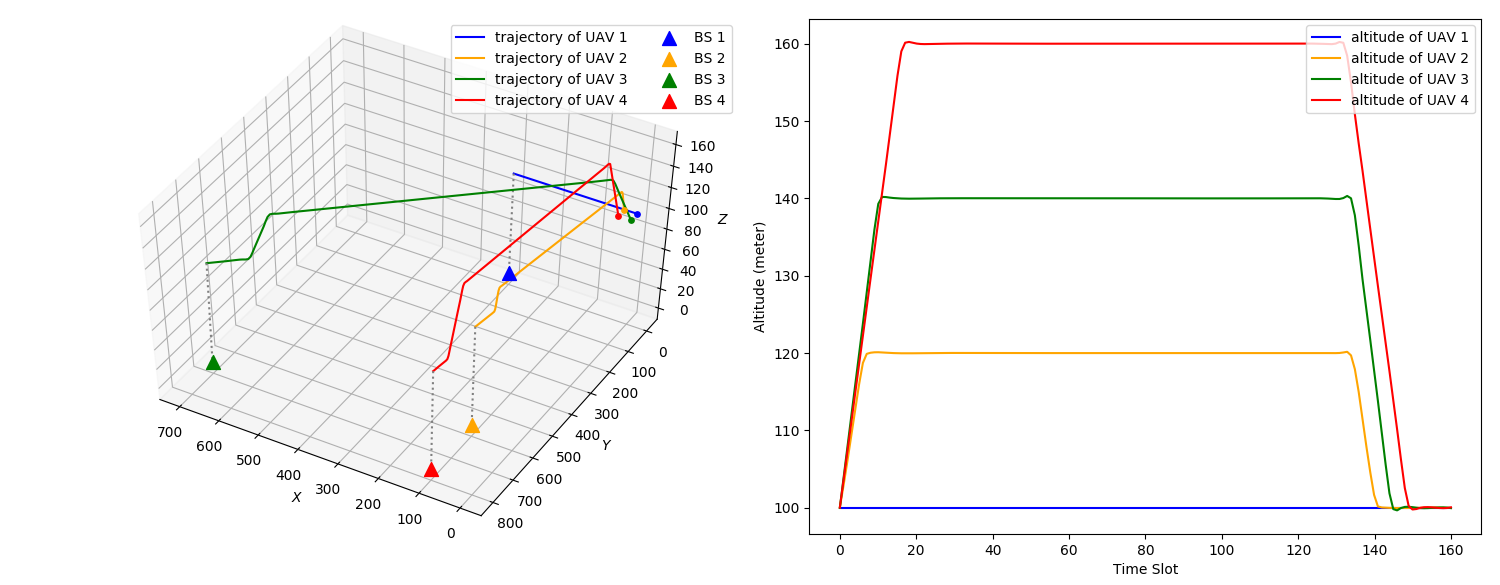
\includegraphics[width=.9\linewidth]{init_trajectory.png}
	\end{figure}
\end{frame}
\begin{frame}
	\frametitle{Simulation Result}
	\begin{itemize}\itemsep-0.5em
		\item Initial trajectory
		\begin{figure}
			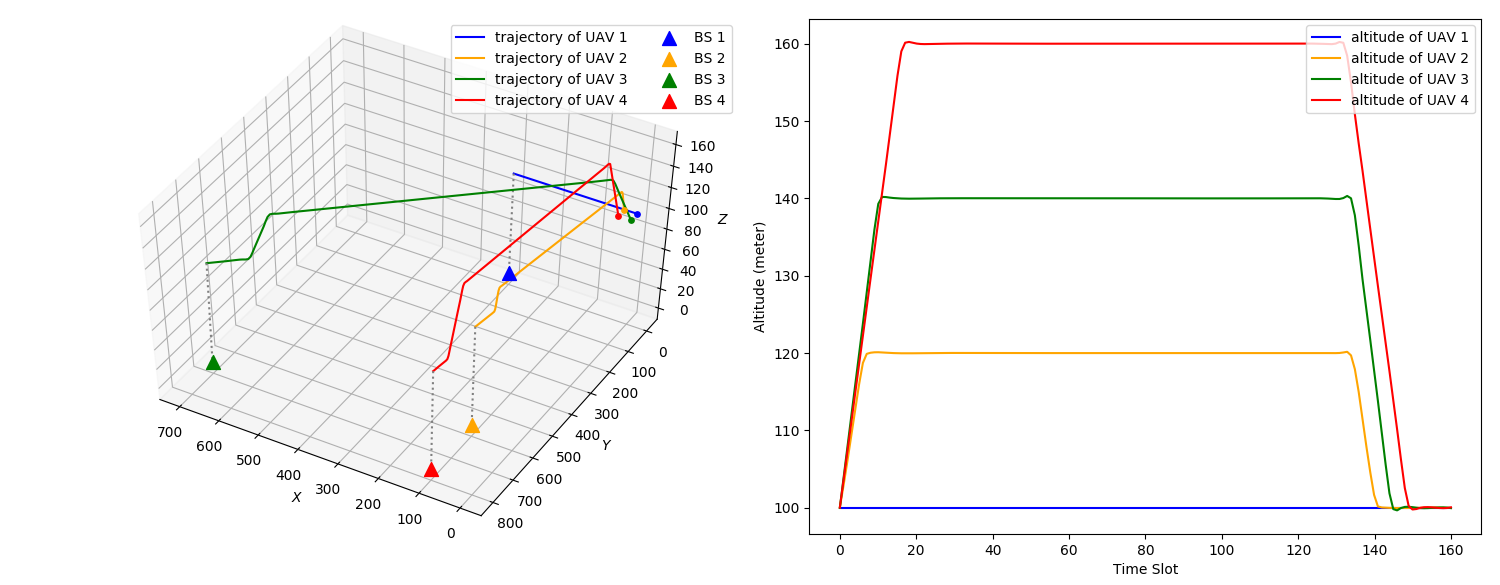
\includegraphics[width=.8\linewidth]{init_trajectory.png}
		\end{figure}
		\item Optimized trajectory
		\begin{figure}
			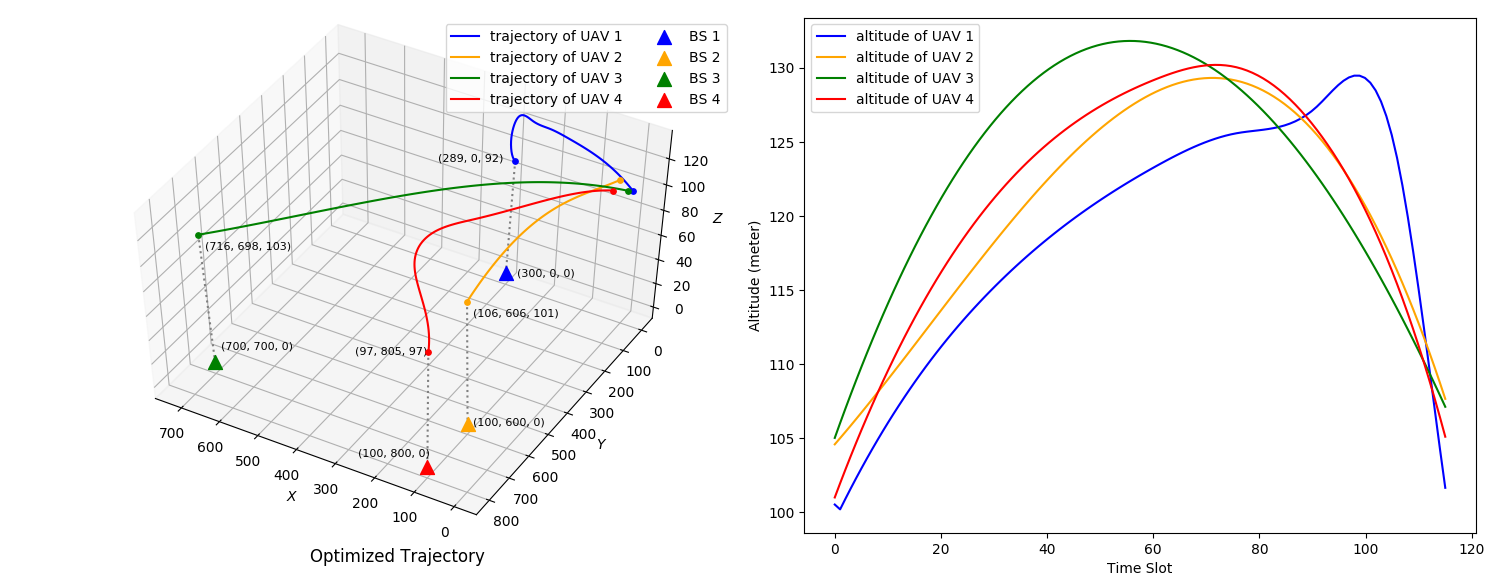
\includegraphics[width=.8\linewidth]{opt_trajectory.png}
		\end{figure}
	\end{itemize}
\end{frame}
\begin{frame}
	\frametitle{Simulation Result}
	\begin{itemize}\itemsep-0.5em
		\item Initial achievable transmission rate
		\begin{figure}
			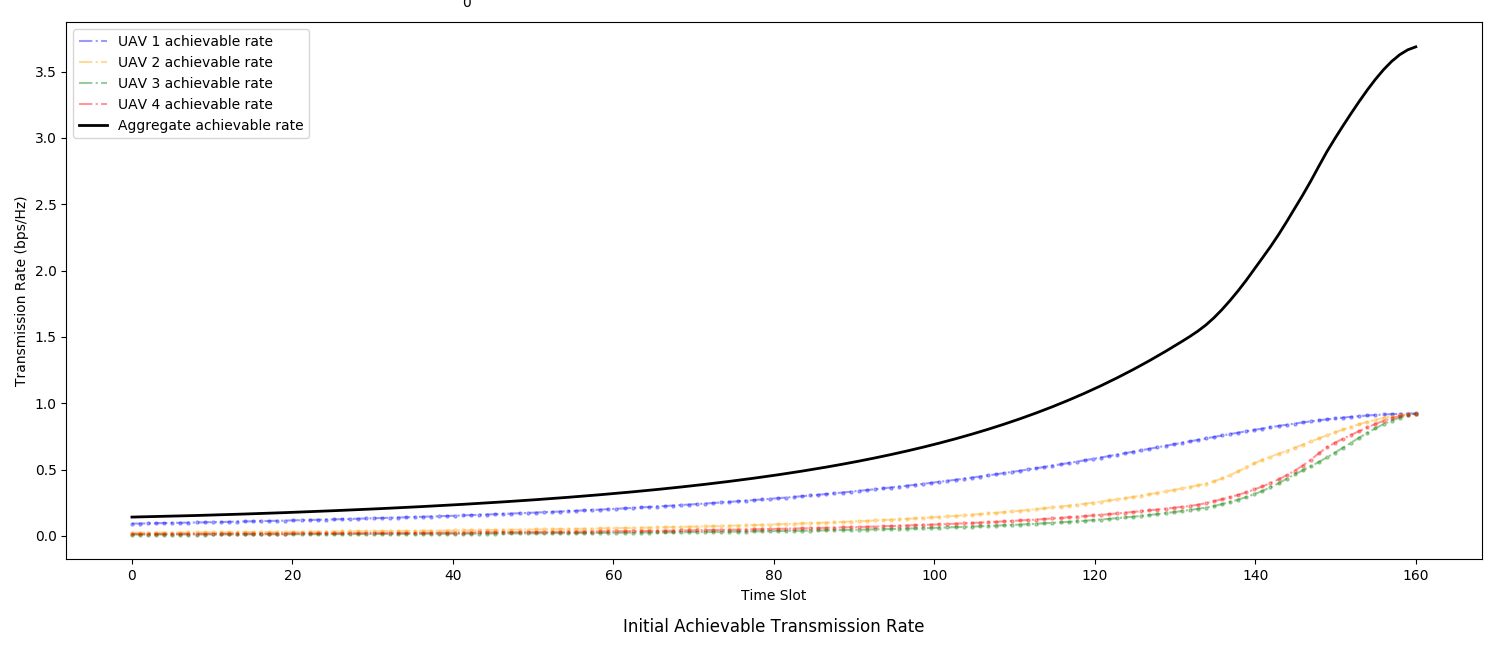
\includegraphics[width=.7\linewidth]{init_rate.png}
		\end{figure}
		\item Optimized achievable transmission rate
		\begin{figure}
			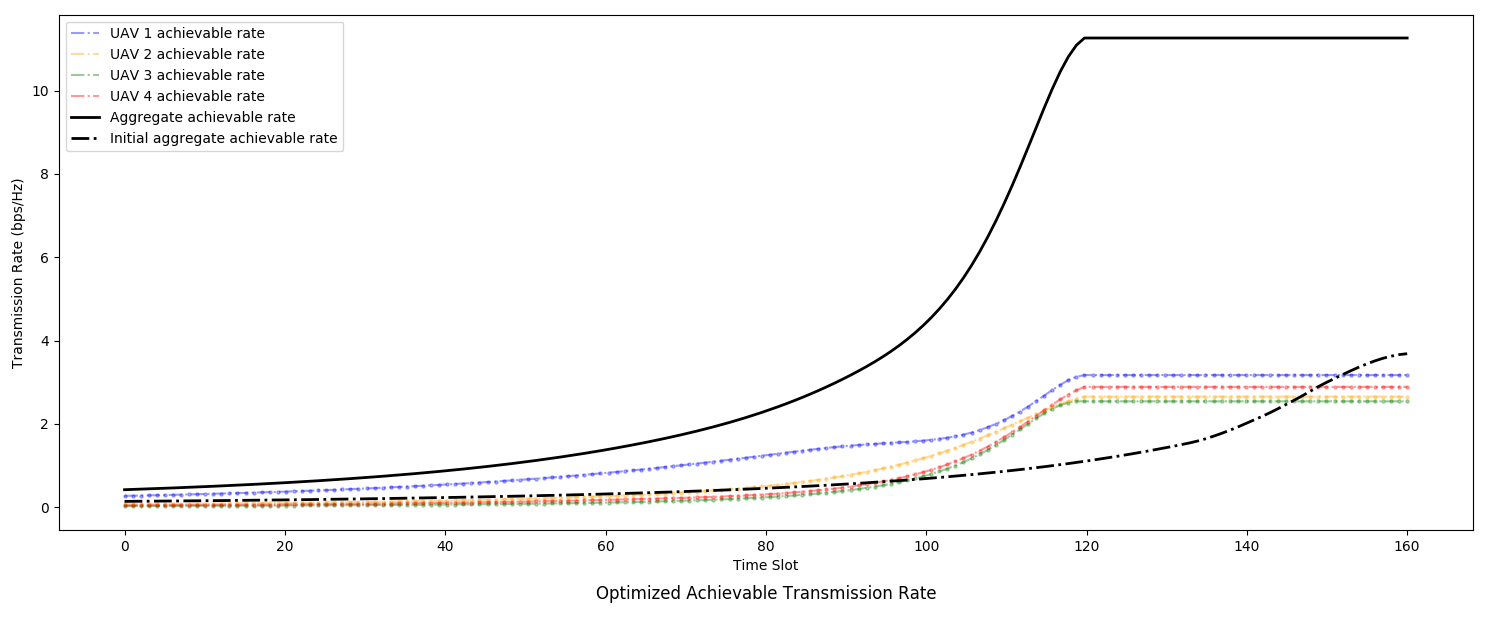
\includegraphics[width=.7\linewidth]{opt_rate.png}
		\end{figure}
	\end{itemize}
\end{frame}

\section{Conclusion}
\begin{frame}
	\frametitle{Conclusion}
	In conclusion, we 
\end{frame}

\begin{frame}{References}
	\bibliographystyle{IEEEtran}
	\bibliography{IEEEabrv,IEEEexample}
\end{frame}

	
	
	
	
	
	
	
\end{document}